\documentclass{standalone}
\usepackage{xr}
\externaldocument{../Chapter1/Section3/Subsection3/Unet}
\begin{document}
\subsection{Training}

This step is one of the most important since the Convolutional Neural Network (CNN) model coming from the training process will be used for the segmentation of the images.\\
Before proceeding with the training, the MRI scans and the medical annotation of each patient were manually checked since for some of them there was misregistration between the image and the medical annotation (i.e. the medical annotation did not correspond to the correct slice).
The medical annotations consist of a set of $(x, y)$ points that border the tumor area on the image.
Pixels inside the bordered area were labeled with a value of 255 while the other ones with 0.
In the end, from 48 patients the remaining ones were 37.
The images were then selected and stored in the proper directories, one for the images in Dicom format and one for the ground-truth images (i.e. medical annotations) stored as 8-bit unsigned integers images.
The training was performed with a custom data generator which was responsible for providing the right input images and ground-truth images, pre-processing them, performing data augmentation, and splitting the images into training and validation sets. 
In particular, a total of 488 images was split for the training (391 images) and validation set (97 images).
Some data augmentation was performed on the training set of data, to overcome the lack of data and to reduce overfitting.
It consisted in adding slightly modified copies of already existing data, using geometrical transformations such as flipping and rotations of the images.
In this particular case, the images were randomly horizontal or vertically flipped.
The ground-truth images were also normalized and rescaled to binary floating-point 32-bit, required to work with \textsc{TensorFlow}\cite{Tensorflow} functions.
\\
In summary, the custom data generator provides the following steps: 
\begin{itemize}
    \item read the input images and ground-truth images from the relative directories
    \item shuffle and split data into training and validation sets
    \item pre-process the input images following the steps described in the previous subsection
    \item normalize and rescale the ground truth images
    \item zip the input images with the correct ground-truth images
    \item perform data-augmentation on training set
\end{itemize} 
An example of input and ground-truth images from the training set is shown in Figure \ref{showdataset}.
As you can see the image size is $512 \times 512$ pixels and the images are horizontal or vertical flip.
The white area on the ground-truth images represents the tumor area.
\\
The network architecture used for this project is a U-Net-like structure made by a contraction and expansion path.
The difference between the original architecture and the one used in this project consists of the use of a so-called \textit{backbone} which refers to the feature extracting network.
Just to clarify this concept, in Figure \ref{fig:unet}, the feature maps (blue boxes) are extracted by a series of Convolutional, ReLu, and Max-pooling layers (denoted by the arrows).
However, one can use various combinations of different layers to extract feature maps. 
So, the combination of layers can create new networks and architectures.
In this case the \textit{backbone} consists of an architecture called \textit{EfficientNetb0}\cite{EfficientNet}.
\\
The loss function used consists of the combination between Dice loss with the binary focal loss\cite{focal}.
The former comes from the Dice coefficient or Dice-Sørensen coefficient (DSC):
\begin{equation}
    1 - DSC = 1 - \frac{2 \mid X \cap Y \mid}{\mid X \mid + \mid Y \mid}
\end{equation}
Where $\mid X \mid$  and $\mid Y \mid$ are the cardinalities of the two sets (i.e. the ground-truth and the prediction).
\\
The latter instead: 
\begin{equation}
    FL = - \alpha y(1 - p(y))^{\gamma}log(p(y)) - \alpha (1 - y) p(y)^{\gamma}log(1 - p(y))
\end{equation}
where $y$ is the the ground-truth, $p(y)$ is the the prediction, $\alpha$ is weighting factor and $\gamma$ a focusing parameter.
\\
Combining the two methods allows for some diversity in the loss.
\\
The algorithm used to minimize the loss function consists of the default \textit{Adam} (Adaptive Moment Estimation) optimizer provided by \textsc{TensorFlow}.
\\
The metric function used to judge the performance of the trained model is the Dice coefficient (DSC), which was the most used in literature for this purpose, thus for having a metric of reference.

\begin{figure}[htp]

    \centering
    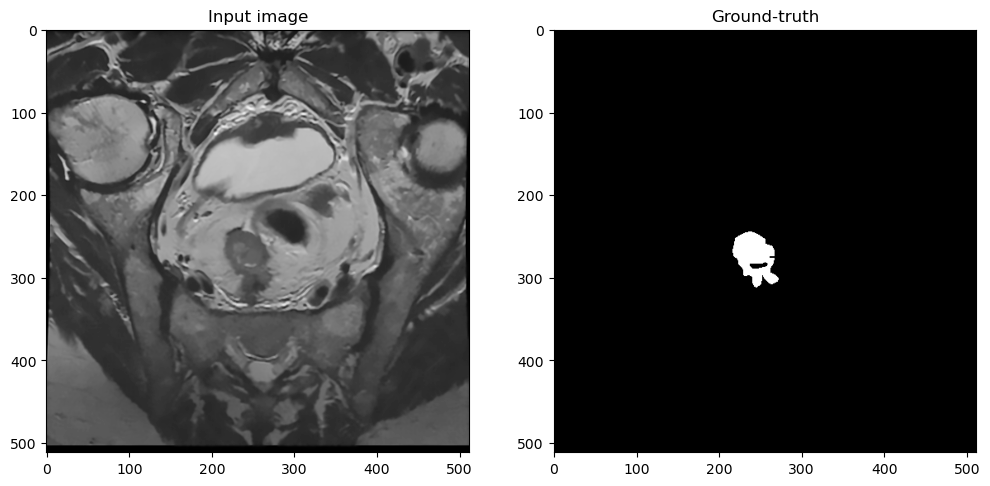
\includegraphics[width=0.9\textwidth]{../images/showdataset.png}
    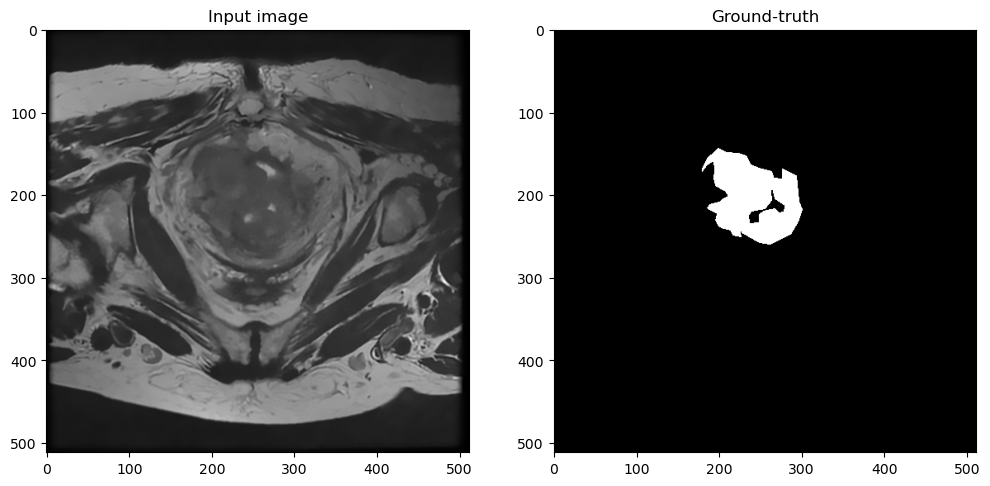
\includegraphics[width=0.9\textwidth]{../images/showdataset1.png}

    \caption{Example of input and ground-truth images from the training set. The images are randomly horizontal or vertical flipped. 
    The white area on the ground-truth images represents the tumor area.}
    \label{showdataset}
    
    \end{figure}

\begin{figure}[htp]

    \centering
    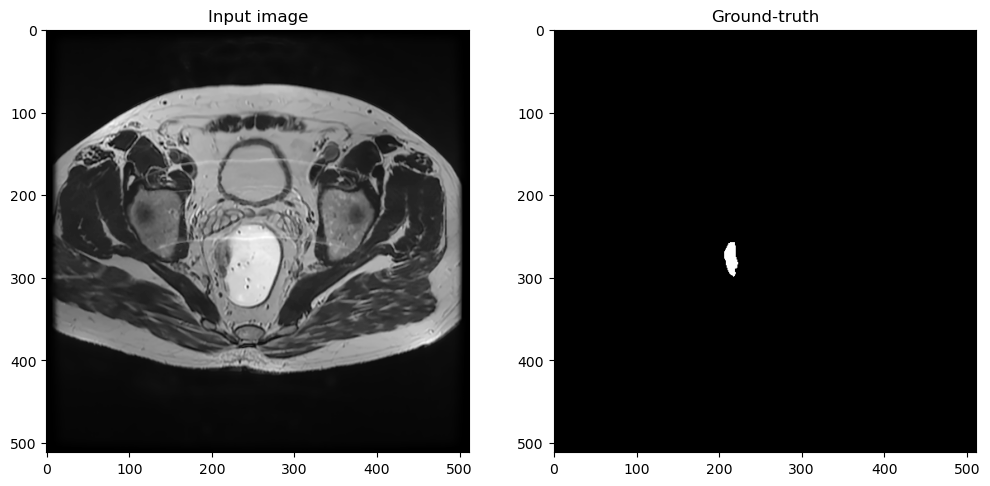
\includegraphics[width=0.9\textwidth]{../images/showdataset2.png}
    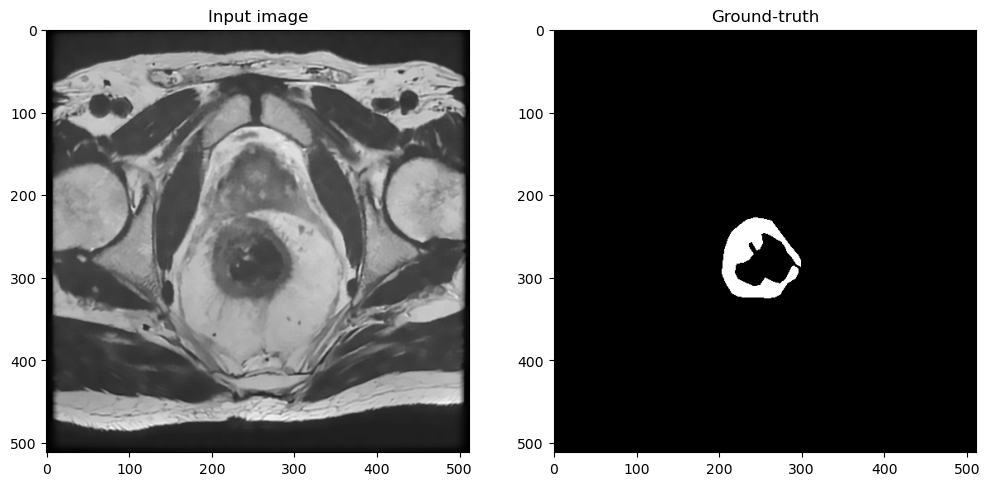
\includegraphics[width=0.9\textwidth]{../images/showdataset3.png}

    \caption{Example of input and ground-truth images from the validation set.
    The white area on the ground-truth images represents the tumor area.}
    \label{showdataset2}
    
    \end{figure}

\end{document}

